\documentclass[12pt]{article}
\usepackage[margin=1in]{geometry}
\usepackage{amsmath,amssymb}
\usepackage{graphicx}
\usepackage{booktabs}
\usepackage{array}
\usepackage{natbib}
\usepackage[small]{caption}
\usepackage{hyperref}
\usepackage{xcolor}

\graphicspath{{figures/}}
\hypersetup{colorlinks=true,linkcolor=blue!60!black,citecolor=blue!60!black,urlcolor=blue!60!black}

\newcommand{\Rtwo}{\ensuremath{R^2}}
\newcommand{\mae}{\ensuremath{\mathrm{MAE}}}
\newcommand{\fl}{Gemini 2.5 Flash Lite}
\newcommand{\gthree}{Gemini 3 Flash}

\title{Is more thinking always better? Think again:\\
\large Less reasoning, better sensory predictions in sensometrics}

\author{
John M. Ennis\\
\textit{Aigora, Richmond, Virginia, USA}
\and
Thierry Worch\\
\textit{FrieslandCampina}
\and
Benjamin Mahieu\\
\textit{Oniris Nantes}
}

\date{Working draft, May 2026}

\begin{document}
\maketitle

\begin{abstract}
Larger and more deliberative language models are often assumed to be better scoring instruments. That assumption may fail when the target response is sensory, affective, and fast. We tested this idea in a consumer cooked-ham study where the task was to score how closely each evaluated product matched each consumer's own ideal product. The data came from a published Ideal-Free-Comment study: 2,758 home-use evaluations from 483 French consumers across 30 commercial cooked hams. Consumers described actual products and their ideal ham using Free-Comment across visual appearance, texture, and flavor, then rated liking on a 0--10 visual analogue scale. For each evaluation, a large language model compared actual and ideal comments and returned structured Likert alignment scores. Those scores were used to predict liking under consumer-group holdout validation. A raw embedding cosine-similarity baseline performed poorly, with \Rtwo{} near 0.20 and \mae{} near 1.83. Direct LLM alignment scoring improved prediction substantially. In the primary analysis, \fl{}, a non-thinking direct-response model, reached \Rtwo{} = 0.573 and \mae{} = 1.22 with a six-point scale and temperature 0.7; bootstrap validation gave mean \Rtwo{} = 0.504. Reasoning-oriented \gthree{} configurations were slower, less accurate, and more prone to structured-output failures. Topic-level validation recovered the published modality hierarchy, with flavor strongest, texture second, and visual appearance weakest. The findings support a model-cognition fit hypothesis: for sensory and consumer scoring tasks, non-thinking models can be better matched to the fast judgment process being measured, while reasoning models may add cost and noise.
\end{abstract}

\noindent\textbf{Keywords:} Free-Comment; Ideal-Free-Comment; sensory analysis; consumer liking; large language models; TabPFN.

\section{Introduction}

Consumers do not usually decide whether they like a food by reasoning through a long checklist. They see it, taste it, feel its texture, and react. Some of that reaction can be described after the fact, but the underlying judgment is fast, sensory, and affective. This matters for large language model (LLM) assisted sensory analysis. If the target human response is closer to fast judgment than deliberate reasoning, a fast direct-response model may be a better scoring instrument than a reasoning-oriented model.

This is the central hypothesis of the paper. Model choice should depend on the cognitive shape of the task. Reasoning models are designed to spend more compute on internal deliberation. That helps when the task requires multi-step inference, proof, planning, or code. Sensory and consumer scoring tasks are different. The model is not solving a puzzle. It is judging whether a product experience matches a consumer's ideal. In that setting, extra deliberation may turn into over-analysis, schema drift, or calibration noise.

There is also a practical reason to care. Consumer research trades off speed, cost, and evidence quality. LLM scoring does not remove this tradeoff. It changes where the tradeoff lands. A reasoning model may look attractive because it sounds more capable, but if it is slower, more expensive, less accurate, and more likely to break schema, it moves the tradeoff in the wrong direction.

The empirical setting is consumer sensory research, where the measurement problem is already difficult. Structured methods such as Check-All-That-Apply (CATA), Just-About-Right scales, and the Ideal Profile Method give analysts clean tables, but they impose a vocabulary in advance. Free-Comment methods do the opposite. They let consumers use their own words. That makes the data closer to the consumer's own experience, but it creates a text-processing problem before the data can be modeled.

Free-Comment has a clear place in sensory science. \citet{tenkleij2003freecomment} introduced open-ended response analysis as a complement to preference mapping. \citet{symoneaux2012comments} showed how comments about likes and dislikes could support preference analysis. \citet{mahieu2020fcwine} found that Free-Comment outperformed CATA for consumer wine characterization in a home-use setting. \citet{mahieu2021mrca} then developed a multiple-response chi-square framework and Multiple-Response Correspondence Analysis (MR-CA) for these data.

Ideal-Free-Comment (IFC) extends the idea. In the cooked-ham study of \citet{mahieu2022ifc}, consumers described the actual hams they evaluated and later described their ideal ham, using the same three sensory modalities: visual appearance, texture in mouth, and flavor. The method is related to the Ideal Profile Method \citep{worch2013ipm}, but it avoids a fixed attribute list. Instead of rating ideal intensity on preselected descriptors, consumers write the ideal in their own language.

That paired design creates an opportunity. If each consumer gives both actual and ideal comments, the central comparison is not simply whether a descriptor appears. It is whether the actual product matches that consumer's ideal experience. The original \citet{mahieu2022ifc} workflow answered this with a classical text-processing pipeline. French comments were cleaned, lemmatized, grouped into latent descriptors, filtered by citation frequency, and cross-tabulated by consumer and product. Descriptor presence was then linked to liking with mixed models, and product-by-descriptor structure was mapped with MR-CA.

This paper asks whether an LLM can score part of that relationship more directly, and whether the best scorer is a non-thinking model. Rather than converting comments to descriptor-presence matrices, we ask the model to compare actual and ideal comments and return sensory alignment scores. The resulting features are small, interpretable, and ready for tabular prediction.

The paper has five research questions:
\begin{enumerate}
\item Are non-thinking LLMs better suited than reasoning-oriented LLMs for sensory actual-versus-ideal scoring?
\item Can direct LLM alignment scores predict consumer liking better than raw embedding similarity?
\item Do the resulting features recover the sensory hierarchy reported by \citet{mahieu2022ifc}?
\item Can model choice improve accuracy, speed, and structured-output reliability at the same time?
\item How should this scoring approach be positioned relative to Free-Comment analysis, IFC, and Semantic Similarity Rating?
\end{enumerate}

\section{Related work}

\subsection{Free-Comment, Ideal-Free-Comment, and MR-CA}

Free-Comment methods collect open-ended sensory descriptions without forcing consumers into a pre-established list of terms. This is useful because consumers may mention attributes that analysts would not have selected in advance. It also avoids problems of list-based methods, including vocabulary restriction, awareness effects, dumping effects, and acquiescence bias.

The cost is preprocessing. Free comments must be cleaned, normalized, grouped, and transformed into structured variables. \citet{mahieu2020fcwine} showed the value of Free-Comment in practice by finding that it outperformed CATA in a home-use wine study on discrimination power and stability of product characterization. \citet{mahieu2021mrca} then formalized analysis of these data with a multiple-response chi-square framework and MR-CA. This matters here because the original cooked-ham analysis is a statistical analysis of multiple-response descriptor data, not a collection of word counts.

IFC, used in the cooked-ham case study of \citet{mahieu2022ifc}, adds the consumer's own ideal product description. Existing products cover only part of the sensory space, and a consumer's ideal may lie outside the product set. \citet{mahieu2022ifc} showed that drivers of liking and ideal-product descriptions provide complementary information, and that ideal descriptions can reveal consumer segments.

\subsection{Text mining and LLM scoring}

Text mining has been used in sensory science for lexicon development, descriptor extraction, term grouping, and analysis of reviews or open comments \citep{hamilton2020nlp,miller2021whisky,hamilton2025review}. Work on automated preprocessing and annotated Free-Comment benchmark data treats preprocessing as a methodological variable rather than a housekeeping step \citep{visallimahieu2023preprocessing,visalli2024madeleines}. This supports a practical reason for direct alignment scoring: a constrained model prompt may reduce some analyst-dependent preprocessing decisions, although it creates its own audit burden around prompting, calibration, and model versioning.

LLMs are now often used as judges, annotators, or semantic scorers. Work such as \citet{zheng2023judge}, \citet{liu2023geval}, and \citet{gilardi2023chatgpt} shows that LLM evaluation and annotation can be useful, but not automatically reliable. Known issues include positional bias, verbosity bias, self-enhancement bias, calibration problems, and task-specific disagreement with human raters. In sensory and consumer research, recent work has considered generative AI across concept, design, and testing phases \citep{motoki2025genai}, coffee flavor annotation \citep{jakkaew2026coffee}, flavor-pairing creativity \citep{wang2025flavor}, and exploratory use of ChatGPT as a sensory evaluator \citep{torrico2025chatgpt}.

Our use case is narrower than general LLM judging. The model does not rank open-ended product concepts or evaluate arbitrary prose. It receives a fixed comparison task, fixed sensory modalities, a fixed scale, and a strict JSON schema. That narrower setup makes the method easier to audit, but it does not remove the need for validation.

\subsection{Semantic Similarity Rating}

Semantic Similarity Rating (SSR) is an important adjacent method, but it is not the method used here. In the approach of \citet{maier2025ssr}, the LLM produces free-text responses. Those responses are mapped to Likert probability distributions by comparing response embeddings to reference anchor statements. SSR therefore returns a probability mass function over the scale.

Our pipeline asks the model directly for integer alignment scores. It is simpler, cheaper, and easy to parse, but it does not provide the distributional information that SSR can provide. Direct numeric scoring can also compress response variation if the model overuses the middle of the scale. We call the method direct LLM alignment scoring.

\subsection{Reasoning models and task fit}

Chain-of-thought prompting and reasoning-oriented models improve many tasks that require explicit decomposition \citep{wei2022cot}. More recent work also shows that extra reasoning can hurt performance on some tasks. \citet{gema2025inverse} report inverse scaling with test-time compute in settings where irrelevant content, spurious features, or loss of focus can mislead a model. \citet{zhou2026reasoning} analyze cases where extended reasoning changes an initially correct answer into an incorrect one. \citet{liu2024cotperceptual} report that chain-of-thought can reduce performance on pattern-matching or perceptual tasks. \citet{sui2025overthinking} review efficient reasoning and overthinking more broadly.

We use System 1 and System 2 as a task-fit analogy, not as a literal claim about model internals \citep{kahneman2011thinking}. Non-thinking models are System-1-like in the operational sense that they return direct answers without extended deliberation. Reasoning models are System-2-like in the operational sense that they spend more compute on intermediate reasoning. The empirical claim is that direct sensory alignment scoring appears to fit the first mode better than the second in this dataset.

\subsection{Tabular foundation models}

TabPFN is a tabular foundation model trained on more than 100 million synthetic tabular tasks generated from structural causal model priors \citep{hollmann2025tabpfn}. It performs prediction on a new tabular dataset through in-context inference rather than ordinary hyperparameter search. This makes TabPFN a good fit for the present workflow. The LLM produces compact tabular features, and TabPFN predicts liking without the tuning burden that would complicate large grid searches and bootstrap validation.

\section{Material and methods}

The case study uses the cooked-ham data of \citet{mahieu2022ifc}, with the open dataset documented by \citet{visalli2024hamdata}. The study included 483 French consumers from seven cities. Consumers purchased and evaluated cooked hams at home over 13 weeks. The product set contained 30 commercial cooked hams selected to cover variation in fat and salt content in the French market. The set excluded smoked, braised, spit-roasted, flavored, and rind-on products.

Each consumer evaluated one or more hams. In the original paper, consumers evaluated between 1 and 14 hams, with a mean of 5.71. The source workbook used here contains 2,758 product evaluations. For each evaluation, consumers described the product by visual appearance, texture in mouth, and flavor. They then rated overall liking on a 0--10 visual analogue scale. At the end of participation, consumers described their ideal ham using the same three modalities.

\begin{table}[ht]
\centering
\caption{Cooked-ham dataset used in the present analysis.}
\label{tab:data}
\begin{tabular}{ll}
\toprule
Quantity & Value \\
\midrule
Consumers & 483 French consumers \\
Products & 30 commercial cooked hams \\
Evaluations & 2,758 home-use evaluations \\
Product period & 13 weeks \\
Liking measure & 0--10 visual analogue scale \\
Text fields & Actual and ideal comments for visual, texture, and flavor \\
Original source & \citet{mahieu2022ifc}; open data article by \citet{visalli2024hamdata} \\
\bottomrule
\end{tabular}
\end{table}

Mahieu et al. processed actual-product Free-Comment data separately by sensory modality. The French text was cleaned, lemmatized, filtered, and grouped into latent descriptors. Descriptors were retained when they were cited in at least 5\% of evaluations for at least one product. The retained descriptors were cross-tabulated by consumer and product, giving a descriptor-presence matrix.

The original paper then linked descriptor presence to liking with a mixed model. Liking was modeled as a function of product, descriptor presence, and consumer, with product and descriptor effects as fixed effects and consumer as a random effect. Descriptor loadings were interpreted as estimates of the effect of citing a descriptor on liking. Positive flavor descriptors such as fragrant, smoked, and ham taste increased liking. Negative descriptors such as insipid, elastic or rubbery, dry or pasty, and visible fat decreased liking. The broad hierarchy was clear: flavor had the strongest relation to liking, texture followed, and visual appearance was weaker.

Ideal-product descriptions were analyzed by descriptor citation proportions. Mahieu et al. also used MR-CA by modality on product-by-descriptor citation proportions, projected the ideal product as a supplementary observation, and projected mean liking as a supplementary variable. This original method is the reference point for our validation. We do not try to reproduce every descriptor effect. We ask whether direct LLM alignment scoring recovers the main sensory structure and predicts liking.

\subsection{LLM scoring and prediction pipeline}

\subsubsection{Direct LLM alignment scoring}

For each consumer-product row, the LLM receives six text fields: ideal visual comment, ideal texture comment, ideal flavor comment, actual visual comment, actual texture comment, and actual flavor comment. In the primary three-feature version, the LLM returns three integer alignment scores: visual alignment, texture alignment, and flavor alignment. A higher score means the actual product was judged closer to that consumer's ideal for that modality.

The prompt framed the model as a sensory and consumer scientist conducting consumer research on ham products. It asked the model to compare a consumer's actual ham experience with the same consumer's ideal ham experience and to score the alignment separately for visual appearance, texture, and flavor. The prompt explicitly instructed the model to focus only on sensory descriptions of the ham itself, to ignore non-sensory comments, and noted that responses came from French consumers and were written in French. The observed liking score was never shown to the model.

For the main six-point version, the scale anchors were: 1 = extremely different, 2 = very different, 3 = somewhat different, 4 = somewhat similar, 5 = very similar, and 6 = extremely similar. The four- and eight-point runs used the same logic with fewer or more granularity levels. The required response format was JSON only:
\[
\{\texttt{"visual"}: X,\ \texttt{"texture"}: X,\ \texttt{"flavor"}: X\}.
\]
Responses were parsed as JSON, coerced to integers, and accepted only when all three fields were present and all scores were within the allowed range. If direct JSON parsing failed, a regex fallback attempted to recover the three named scores. Rows that still failed parsing were counted as structured-output failures. Missing comments were passed as \texttt{(empty)} rather than silently removed.

The method changes the estimand relative to descriptor-presence analysis. \citet{mahieu2022ifc} estimate how the presence of a descriptor is associated with liking. We estimate how close the actual sensory experience is to the consumer's ideal. These are related, but not identical. Because of that difference, signed descriptor coefficients should not be directly compared with our feature importances. The correct comparison is broader structure: modality order, topic rank agreement, and predictive signal.

\begin{figure}[ht]
\centering
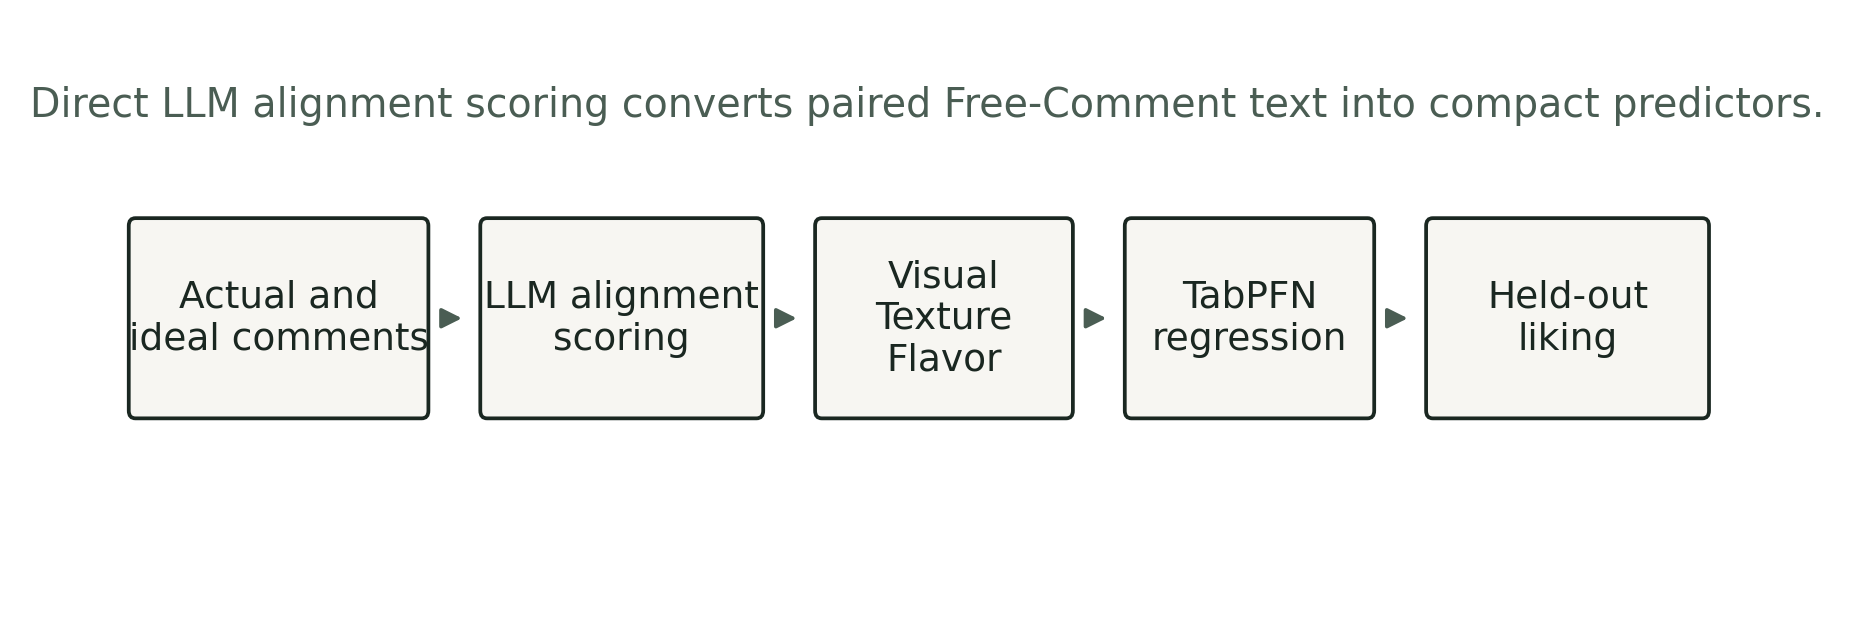
\includegraphics[width=0.95\textwidth]{fig1_workflow.png}
\caption{Direct LLM alignment scoring workflow. Paired actual and ideal Free-Comment fields are scored by sensory modality, then used as compact predictors of held-out liking.}
\label{fig:workflow}
\end{figure}

\subsubsection{Model grid and validation}

The model grid tested the paper's central hypothesis. If sensory alignment scoring behaves like a fast judgment task, non-thinking models should score it well. If extra reasoning improves the measurement, \gthree{} thinking configurations should outperform Flash Lite. The presentation analysis described a 27-configuration grid: three model configurations by three scale granularities by three temperatures. The core task, JSON schema, dataset, and downstream evaluation procedure were held fixed.

\begin{table}[ht]
\centering
\caption{Experimental factors in the LLM scoring grid.}
\label{tab:grid}
\small
\begin{tabular}{p{0.18\textwidth}p{0.36\textwidth}p{0.36\textwidth}}
\toprule
Factor & Levels varied & Held fixed \\
\midrule
Model & \fl{}; \gthree{} minimal; \gthree{} low & Prompt task and JSON schema \\
Scale size & 4-point, 6-point, 8-point Likert scales & Actual-versus-ideal comparison \\
Temperature & 0.0, 0.3, 0.7 & topP, topK, candidate count \\
Validation & Grouped consumer holdout; 200 bootstrap resamples & No consumer leakage between train and test \\
\bottomrule
\end{tabular}
\end{table}

The validation split grouped rows by consumer. This is important because the same consumer can evaluate multiple hams. If rows from one consumer appeared in both train and test data, the estimate could be inflated by consumer-level leakage. We report \Rtwo{}, \mae{}, and root mean squared error where available:
\[
\Rtwo = 1 - \frac{\sum_i (y_i-\hat{y}_i)^2}{\sum_i (y_i-\bar{y})^2},
\qquad
\mae = \frac{1}{n}\sum_i |y_i-\hat{y}_i|.
\]

\subsubsection{Baselines and downstream prediction}

The first baseline used raw text embeddings. Actual and ideal comments were embedded, and cosine similarity was used as a predictor:
\[
\cos(\mathbf{a},\mathbf{i}) =
\frac{\mathbf{a}\cdot\mathbf{i}}{\|\mathbf{a}\|\|\mathbf{i}\|}.
\]
This baseline tested whether generic semantic closeness could solve the task without constrained sensory scoring.

The direct LLM scoring pipeline produced compact tabular features. These features were passed to downstream models to predict liking. The main model in the presentation analysis was TabPFN. Other downstream models were also compared, including XGBoost, Gradient Boosting, Ridge Regression, and Random Forest.

\subsubsection{Topic-level validation}

The primary pipeline uses three alignment scores. To compare more directly with the \citet{mahieu2022ifc} descriptor analysis, we also ran a topic-level version with 17 topic-alignment scores. Topics covered overall visual match, color and pinkness, fat and lean appearance, surface moisture and shine, slice structure, overall texture, tenderness, firmness and rubberiness, dryness and juiciness, fibrous pieces, thickness and chew, overall flavor, saltiness, ham taste, smoky or spiced notes, blandness or insipid intensity, and off-notes or aftertaste.

Each score measures actual-versus-ideal alignment for that topic. These are not descriptor citation counts. To compare them with \citet{mahieu2022ifc}, we mapped each topic to the closest descriptor family from the original analysis and compared normalized strength and rank order rather than raw signed effects. We also created an MR-CA-style topic map by averaging LLM topic-alignment scores by product and running correspondence analysis on the resulting 30 product by 17 topic matrix. This map is a diagnostic analog, not a literal replication of the original MR-CA.

\section{Results}

\subsection{Raw embeddings did not capture the actual-versus-ideal relation}

The embedding baseline performed poorly, with \Rtwo{} near 0.20 and \mae{} near 1.83. This is informative because the task is not simply to decide whether two comments are semantically close. A consumer might describe an actual ham and an ideal ham with overlapping words but different sensory implications. Another consumer might use different words to describe a close match. Raw cosine similarity does not force the comparison to respect modality, hedonic direction, or consumer-specific ideals.

\subsection{Non-thinking alignment scoring improved liking prediction}

The best presentation configuration used \fl{}, no thinking, a six-point scale, and temperature 0.7. It reached \Rtwo{} = 0.573 and \mae{} = 1.22 on the main split. Bootstrap validation produced mean \Rtwo{} = 0.504 with a 95\% interval of [0.429, 0.582].

\begin{table}[ht]
\centering
\caption{Primary predictive and operational results.}
\label{tab:primary}
\footnotesize
\begin{tabular}{@{}p{0.20\textwidth}p{0.10\textwidth}p{0.06\textwidth}p{0.19\textwidth}p{0.06\textwidth}p{0.07\textwidth}p{0.10\textwidth}@{}}
\toprule
Configuration & Scale, temp. & \Rtwo{} & Bootstrap \Rtwo{} & \mae{} & Time (s) & Parse errors \\
\midrule
Embedding baseline & -- & 0.200 & -- & 1.83 & $<5$ & 0\% \\
\fl{} & 6 pt, 0.7 & 0.573 & 0.504 [0.429, 0.582] & 1.22 & 102 & 0.02\% \\
\gthree{} low & 8 pt, 0.7 & 0.518 & 0.462 [0.388, 0.531] & 1.26 & 614 & 0.15\% \\
\gthree{} minimal & 4 pt, 0.7 & 0.411 & -- & 1.38 & 131 & 3.40\% \\
\bottomrule
\end{tabular}
\end{table}

The full grid supports the same conclusion. All nine Flash Lite configurations beat all 18 Gemini 3 Flash configurations on \mae{} in the presentation analysis. Model family accounted for the largest share of performance variation across the grid, ahead of scale granularity and temperature. Bootstrap comparisons favored Flash Lite, with estimated probabilities of 99.3\% versus Gemini 3 minimal thinking and 91.2\% versus Gemini 3 low thinking.

\begin{figure}[ht]
\centering
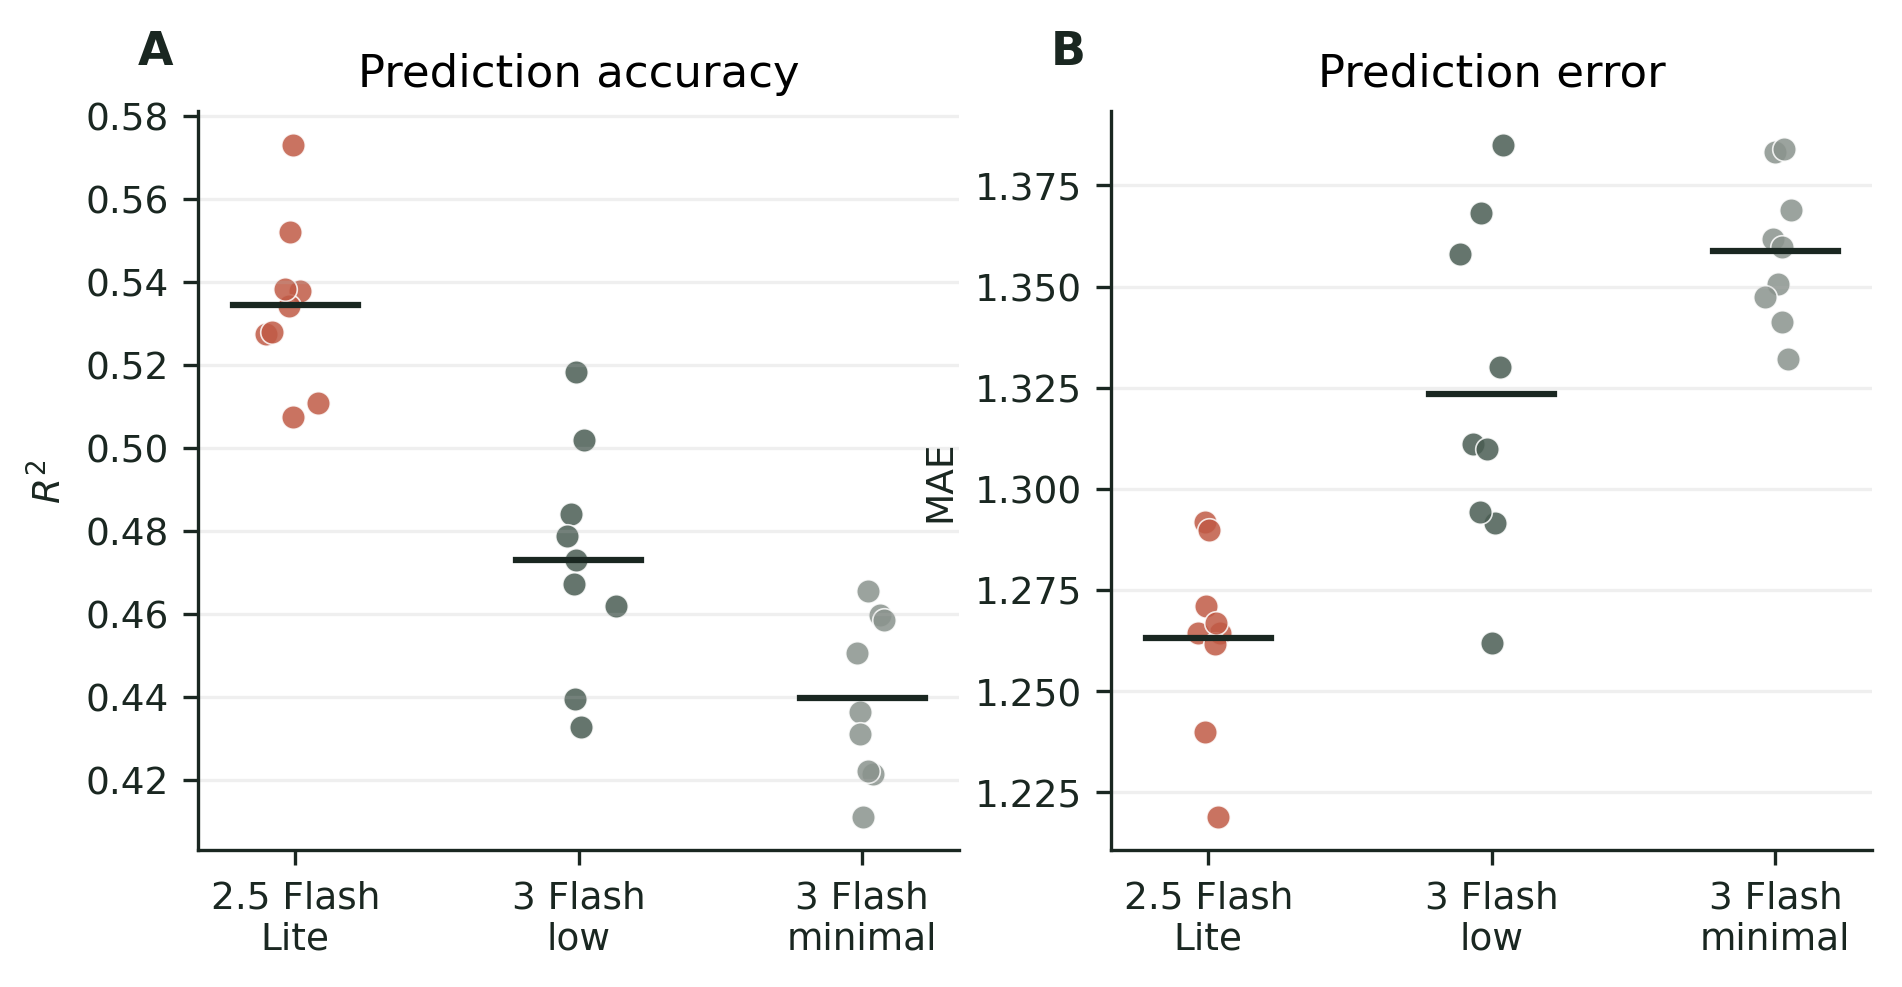
\includegraphics[width=0.92\textwidth]{fig2_model_grid.png}
\caption{Performance across the 27-configuration grid. Points are individual combinations of model, scale size, and temperature. Horizontal bars show model-family means.}
\label{fig:grid}
\end{figure}

\subsection{Reasoning was slower and less reliable}

The tested reasoning-oriented configurations also carried operational costs. Runtime increased sharply for \gthree{} low thinking, and structured-output failures were more frequent for \gthree{} minimal thinking. These failures matter because the pipeline depends on thousands of parseable JSON responses.

\begin{figure}[ht]
\centering
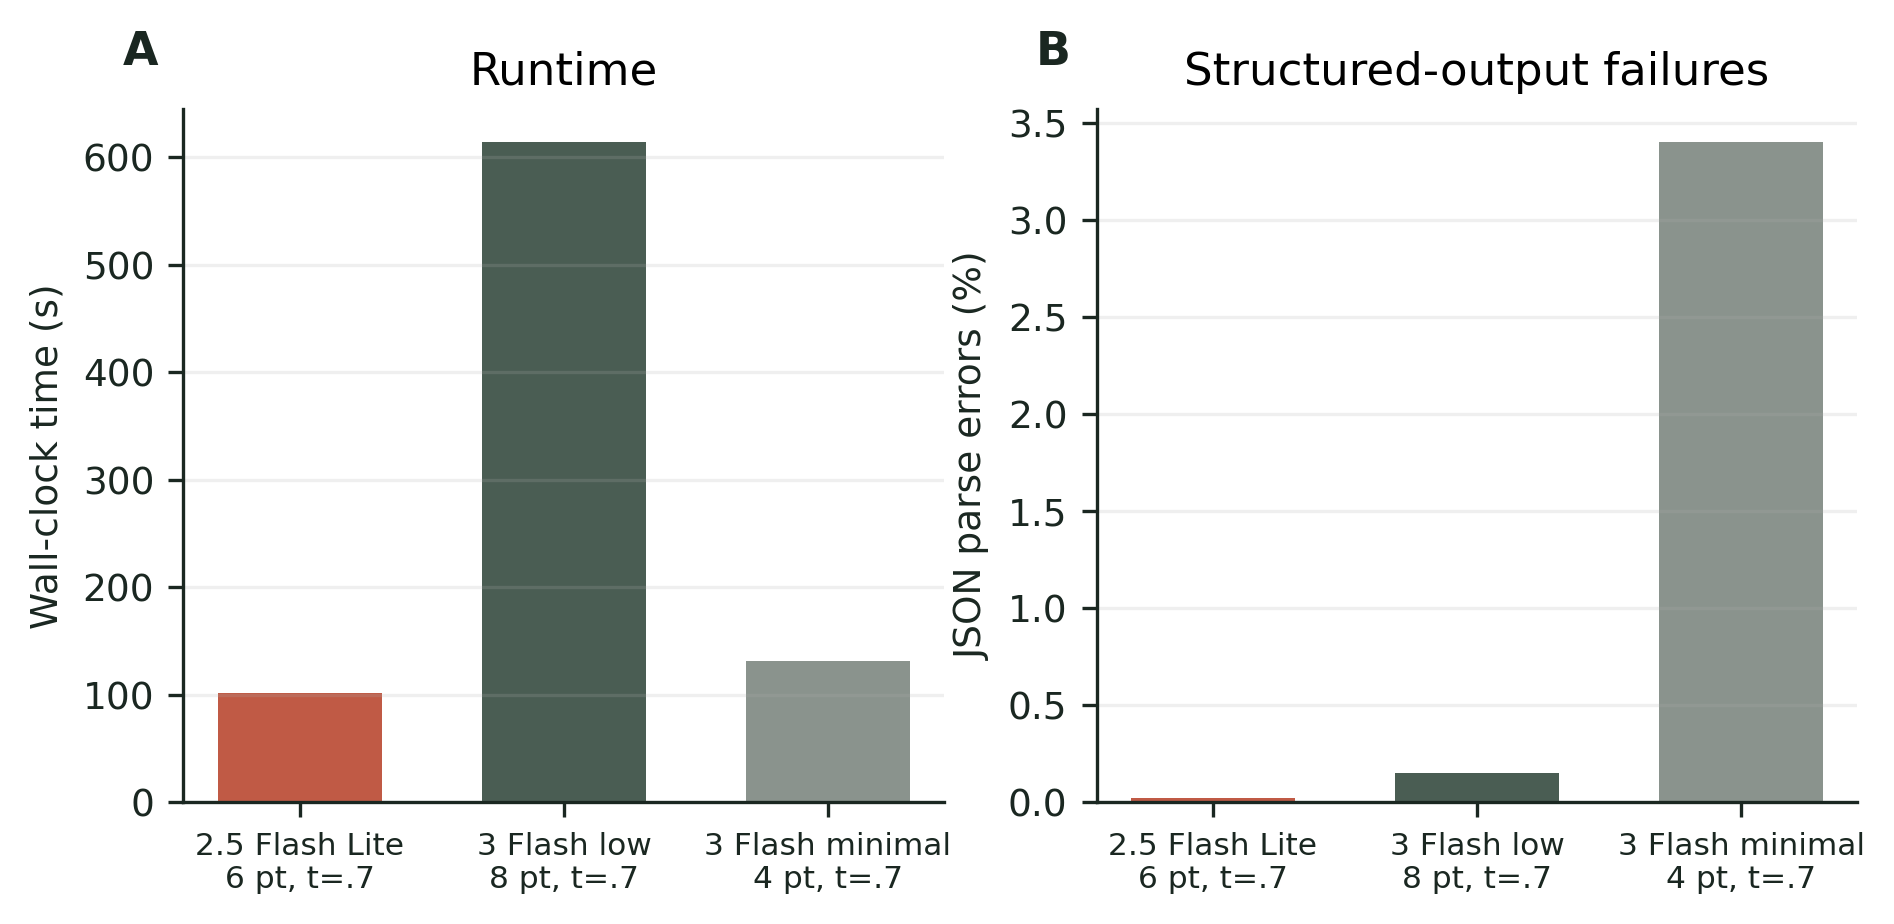
\includegraphics[width=0.92\textwidth]{fig3_operations.png}
\caption{Operational comparison for highlighted configurations. A useful scorer must be accurate, fast enough to run across thousands of rows, and reliable enough to return parseable structured output.}
\label{fig:operations}
\end{figure}

\subsection{Row-level disagreements illustrate the mechanism}

The aggregate result can sound abstract, so we inspected row-level disagreements. In one high-liking case, consumer H041 gave the product a liking score of 8.90. The actual comments included ``The ham breaks apart, but it has a good texture'' and ``Very good, not too salty.'' The ideal comments asked for a slightly thick slice that does not fall apart in the mouth, is not too dry, and has a light smoky taste that is not too salty.

The two models received the same row, prompt, and 1 to 6 scoring scale. Flash Lite scored the row 4, 5, and 6 for visual, texture, and flavor similarity. \gthree{} low thinking scored it 4, 2, and 4. A plausible interpretation is that the reasoning-oriented model penalized a literal texture mismatch, while Flash Lite preserved the high-liking signal in the overall sensory match. These examples do not replace the statistical results. They illustrate how a reasoning-oriented model may over-parse local mismatches in consumer language and convert them into severe similarity penalties, even when actual liking remains high.

\subsection{The sensory hierarchy matched the original study}

The feature-importance analysis from the three-score model gave the largest role to flavor, a smaller role to texture, and the weakest role to visual appearance. This matches the broad pattern in \citet{mahieu2022ifc}.

\begin{figure}[ht]
\centering
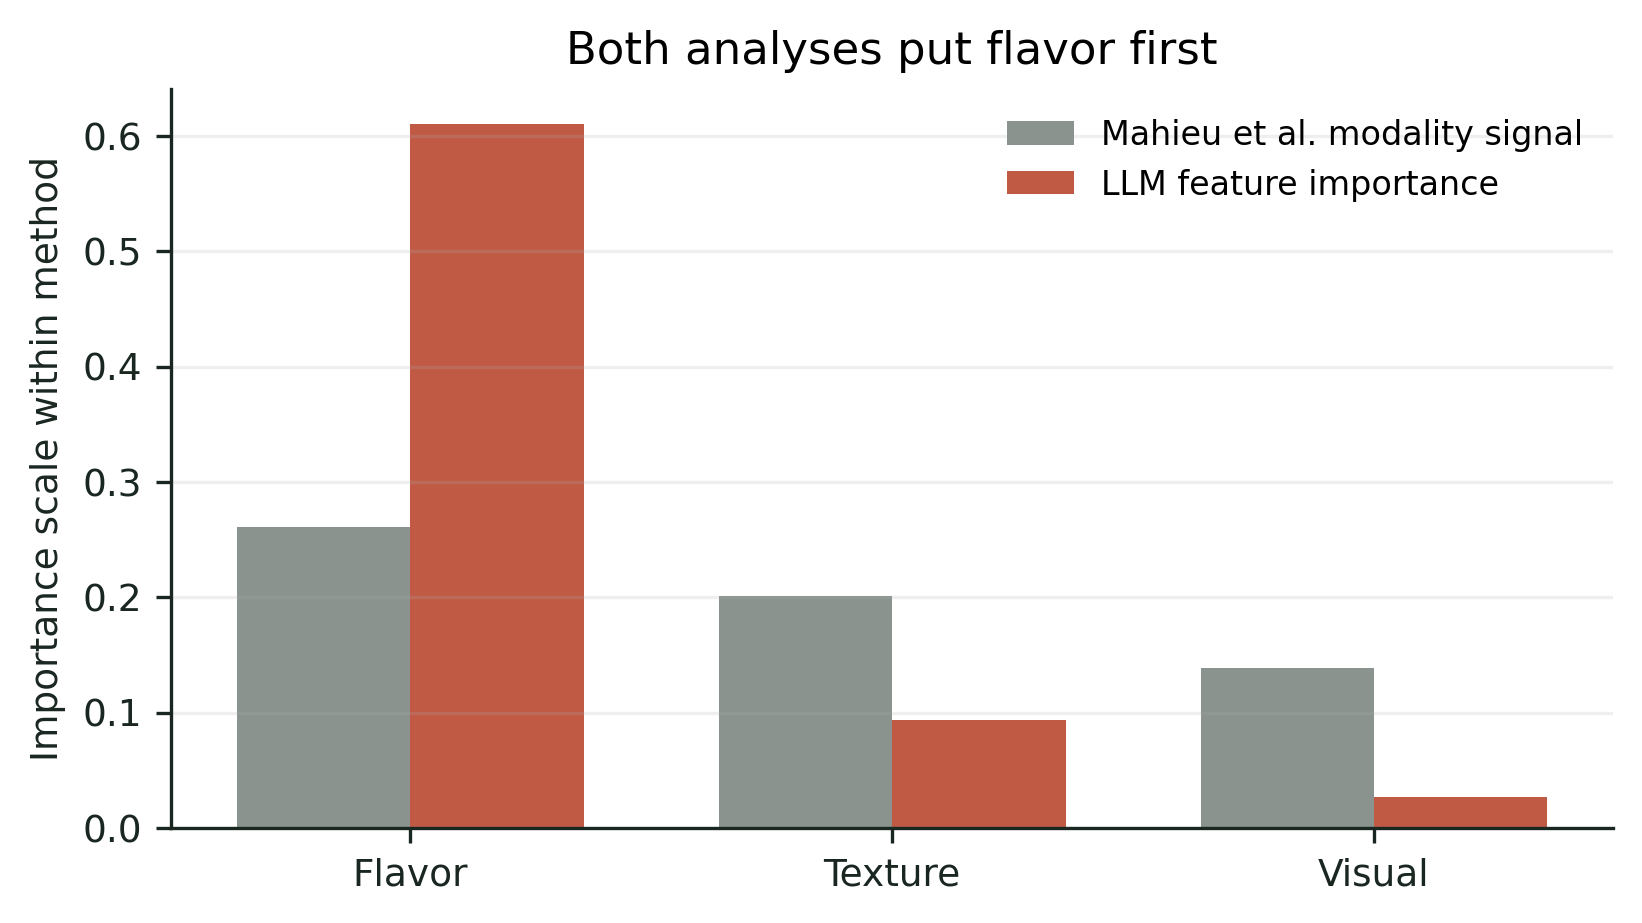
\includegraphics[width=0.78\textwidth]{fig4_modality_importance.png}
\caption{Modality-level sanity check. The two bars are not in the same units: Mahieu et al. values summarize modality signal from the original descriptor-based analysis, while our values are downstream model feature importances from LLM alignment scores. The comparison is about order and structure.}
\label{fig:modality}
\end{figure}

The topic-level analysis strengthened that result. It recovered the same modality order and showed substantial rank agreement across mapped topic families. Across 17 matched topic families, Kendall's $\tau_b$ was 0.519 with a two-sided permutation $p = 0.0033$. Spearman's $\rho$ was 0.715, and 9 of the top 10 topic families overlapped.

\begin{figure}[ht]
\centering
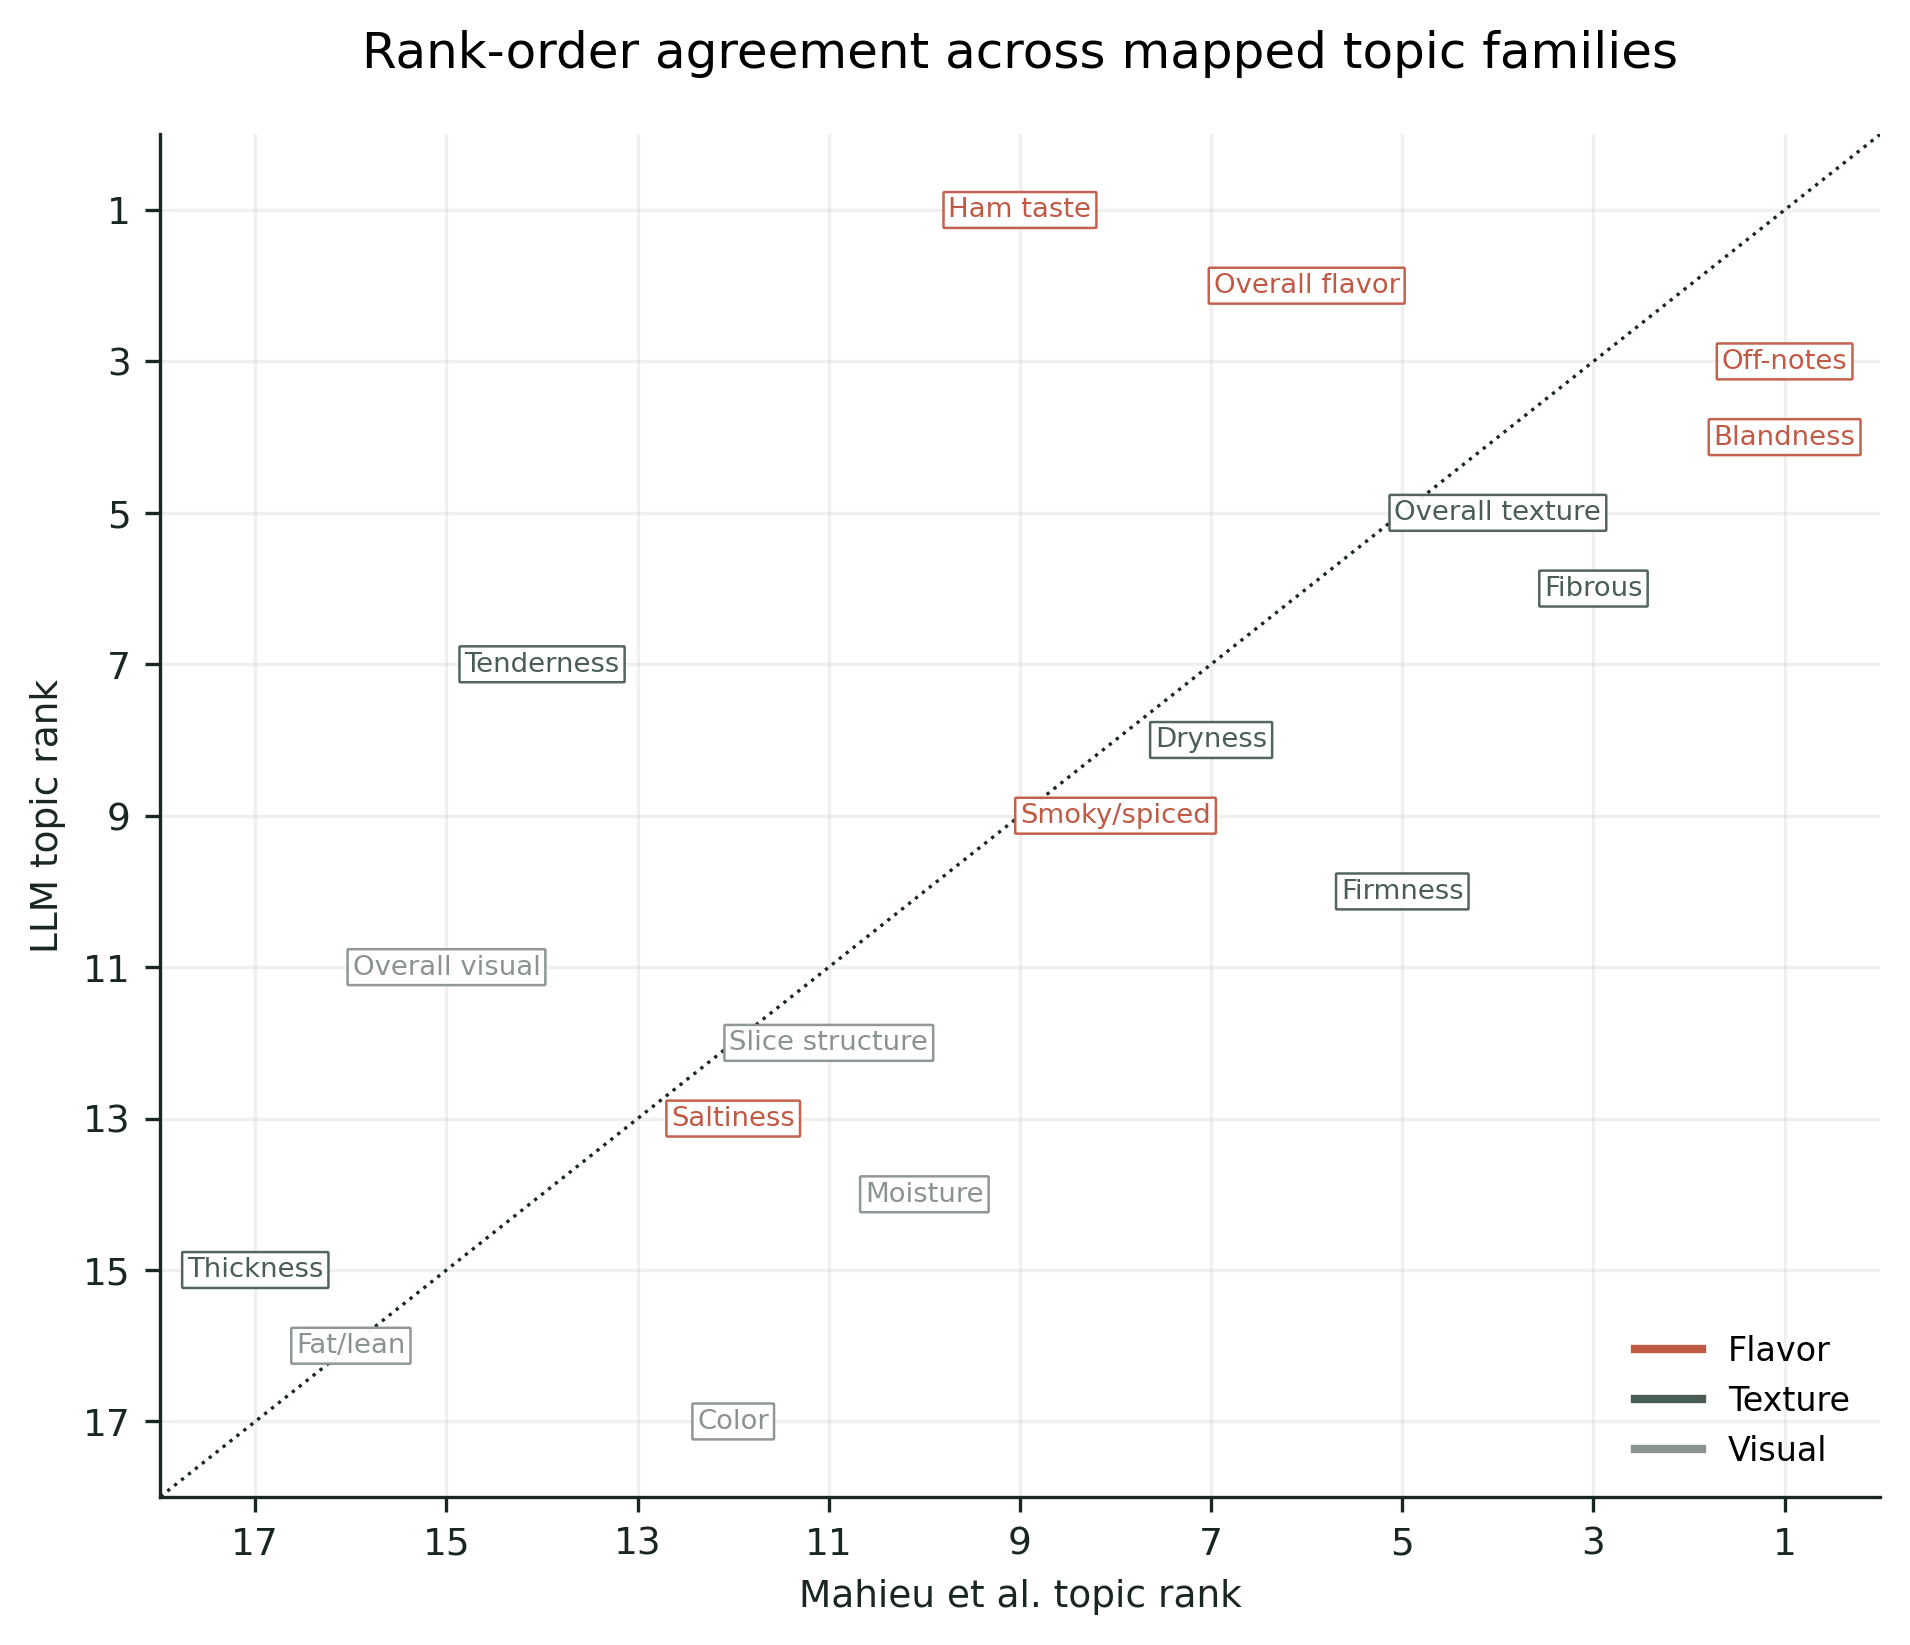
\includegraphics[width=0.72\textwidth]{fig5_topic_rank.png}
\caption{Rank-order comparison between mapped Mahieu et al. descriptor families and LLM topic-alignment families. Lower ranks are stronger. The comparison covers 17 matched topic families; 9 of the top 10 topic families overlapped, with Kendall's $\tau_b = 0.519$ and Spearman's $\rho = 0.715$.}
\label{fig:topicrank}
\end{figure}

\begin{table}[ht]
\centering
\caption{Topic-level validation results.}
\label{tab:topic}
\begin{tabular}{ll}
\toprule
Quantity & Result \\
\midrule
Valid topic-level rows & 2,757 \\
Parse errors & 1 \\
Topic families & 17 \\
Original modality order & Flavor $>$ Texture $>$ Visual \\
LLM modality order & Flavor $>$ Texture $>$ Visual \\
Modality Spearman $\rho$ & 1.000 \\
Topic rank Spearman $\rho$ & 0.715 \\
Topic rank Kendall $\tau$ & 0.519 \\
GB fallback topic prediction & \Rtwo{} = 0.470; \mae{} = 1.367; RMSE = 1.767 \\
\bottomrule
\end{tabular}
\end{table}

\subsection{TabPFN made the full loop practical}

The downstream model comparison was not the headline result, but it matters for the workflow. TabPFN, XGBoost, Gradient Boosting, and Ridge were nearly tied in mean \Rtwo{} across configurations, with Random Forest behind. TabPFN had the best mean \Rtwo{} in the slide analysis at 0.476 and won 74\% of configurations. XGBoost was close at 0.474. The reason for using TabPFN is operational. The accuracy margin was modest, but TabPFN required no separate hyperparameter search and runs as a single tabular forward pass.

\begin{table}[ht]
\centering
\caption{Downstream model comparison across LLM configuration combinations.}
\label{tab:downstream}
\begin{tabular}{lcc}
\toprule
Downstream learner & Mean \Rtwo{} & Configurations won \\
\midrule
TabPFN v2 & 0.476 & 74\% \\
XGBoost & 0.474 & -- \\
Gradient Boosting & 0.473 & -- \\
Ridge Regression & 0.469 & -- \\
Random Forest & 0.444 & -- \\
\bottomrule
\end{tabular}
\end{table}

\section{Discussion}

This study shows that the cognitive style of the scoring model matters. The best-performing scorer was the fast, non-thinking model, not the reasoning-oriented model. That result fits the nature of the target task. Liking a ham is a sensory and affective judgment. The scoring prompt asks the model to judge whether the actual product matched the consumer's ideal experience. It does not ask the model to solve a multi-step reasoning problem.

Direct LLM alignment scoring also turns IFC data into useful predictors of liking. The model receives paired actual and ideal consumer comments, scores sensory alignment, and produces tabular features that can be modeled with standard tools. In the cooked-ham dataset, those features predicted liking much better than raw embedding similarity and recovered the same broad sensory hierarchy as the original descriptor-based analysis.

The result sits between classical sensory statistics and newer LLM judging methods. It does not discard the sensory structure of the problem. The prompt asks for visual, texture, and flavor comparisons, and the topic-level extension uses topic families grounded in the original descriptor analysis. At the same time, it avoids much of the manual work of cleaning, lemmatizing, grouping, and filtering free comments before modeling.

The model-comparison result matters because LLM workflows are often evaluated as if capability were one-dimensional. Here, the best option was also the less deliberative option. Flash Lite gave better prediction, lower runtime, and better output behavior than the tested reasoning-oriented configurations. This supports a task-fit view of model selection. A model that is stronger on formal reasoning may be a worse measurement instrument for a fast sensory scoring task.

The method also changes what is being measured. Descriptor-presence analysis asks what terms were cited and how their presence relates to liking. Alignment scoring asks whether the actual product matched the consumer's ideal. For liking prediction, that relational score may be closer to the consumer decision process. For comparison with classical drivers, it requires care. The correct comparison is not raw signed coefficient matching. It is broader structure, modality order, and rank agreement.

The benchmark should also be treated as a living instrument. Gemini 3.5 Flash launched on May 19, 2026, two days before the Sensometrics presentation. That fact does not weaken the result. It clarifies the duty of the sensometrician: model releases move the baseline, so the scoring grid should be rerun after major model changes. The durable contribution is the benchmark loop and the task-fit hypothesis, not a permanent ranking of model names.

\section{Limitations and future work}

This is a single-product-category study. Cooked ham has a clear sensory structure, and flavor dominates liking in the original analysis. Other categories may have different modality balances and may not favor non-thinking models to the same extent.

The main model comparison is limited to Gemini configurations. The paper should not claim that all reasoning models behave the same way. It should claim that the tested reasoning configurations did not help this sensory scoring task, and that the result supports a broader task-fit hypothesis worth testing.

Exact model aliases require audit. Any use of provider aliases must be resolved to stable model IDs and run dates before submission.

Direct LLM scoring is not proper SSR. SSR may provide better-calibrated distributions and uncertainty information. A fair comparison should ask whether SSR's probability distributions improve calibration or whether direct scoring wins because the prompt focuses the model on the sensory comparison we care about.

The topic-level predictive result currently uses Gradient Boosting as a placeholder. Topic-level TabPFN results should replace it if a stable TabPFN run becomes available.

The topic-level comparison to \citet{mahieu2022ifc} uses mapped descriptor families and approximate driver strengths from processed paper notes. These mappings and values need to be checked against the primary paper or original code before final submission.

Finally, a small synthetic-agent smoke test raised an interesting question about model-person fit: whether some consumers might be better matched to direct-response models and others to reasoning-oriented models. The current smoke test is prompt-sensitive, small, and not tied to the same TabPFN workflow as the main study. It belongs in future work unless redesigned.

\section{Conclusion}

Direct LLM alignment scoring offers a practical way to analyze Ideal-Free-Comment data, but the larger lesson is about model-cognition fit. In the cooked-ham case study, the non-thinking model was the better sensory scorer. It turned paired actual and ideal comments into compact predictors of liking, outperformed raw embedding similarity, and recovered the main sensory hierarchy from the original Free-Comment analysis. The reasoning-oriented configurations were slower, less accurate, and less reliable in structured output. For sensory and consumer analytics, the best LLM is not necessarily the largest or most deliberative one. It is the model whose response style fits the measurement task.

\section*{Declaration of competing interest}

The authors declare no competing interests.

\section*{Declaration of generative AI and AI-assisted technologies in the manuscript preparation process}

During preparation of this working draft, the authors used AI-assisted tools to support literature synthesis, manuscript organization, code generation, figure generation from analysis data, and language editing. The authors reviewed and edited the content and are responsible for the final manuscript.

\section*{Data and code availability}

Data, analysis scripts, generated scoring artifacts, figures, and manuscript build files will be made available in a public GitHub repository at \url{https://github.com/aigorahub/model-cognition-fit-llm-ifc-ham}.

\bibliographystyle{plainnat}
\begin{thebibliography}{99}

\bibitem[Argyle et~al.(2023)]{argyle2023silicon}
Argyle, L. P., Busby, E. C., Fulda, N., Gubler, J. R., Rytting, C., \& Wingate, D. (2023).
Out of one, many: Using language models to simulate human samples.
\textit{Political Analysis}, 31(3), 337--351.
\url{https://doi.org/10.1017/pan.2023.2}.

\bibitem[Brand et~al.(2023)]{brand2023willingness}
Brand, J., Israeli, A., \& Ngwe, D. (2023).
Using LLMs for market research.
Harvard Business School Working Paper 23-062.
\url{https://papers.ssrn.com/sol3/papers.cfm?abstract_id=4395751}.

\bibitem[Gilardi et~al.(2023)]{gilardi2023chatgpt}
Gilardi, F., Alizadeh, M., \& Kubli, M. (2023).
ChatGPT outperforms crowd workers for text-annotation tasks.
\textit{Proceedings of the National Academy of Sciences}, 120(30), e2305016120.
\url{https://doi.org/10.1073/pnas.2305016120}.

\bibitem[Gema et~al.(2025)]{gema2025inverse}
Gema, A. P., H{\"a}gele, A., Chen, R., and colleagues. (2025).
Inverse Scaling in Test-Time Compute.
\textit{Transactions on Machine Learning Research}.
\url{https://doi.org/10.48550/arXiv.2507.14417}.

\bibitem[Hamilton and Lahne(2020)]{hamilton2020nlp}
Hamilton, L. M., \& Lahne, J. (2020).
Fast and automated sensory analysis: using natural language processing for descriptive lexicon development.
\textit{Food Quality and Preference}, 83, 103926.
\url{https://doi.org/10.1016/j.foodqual.2020.103926}.

\bibitem[Hamilton et~al.(2026)]{hamilton2025review}
Hamilton, K., Miller, R. J., \& Lahne, J. (2026).
Sensory applications of natural language processing and text analysis in practice: a review of recent literature.
\textit{Current Opinion in Food Science}, 67, 101370.
\url{https://doi.org/10.1016/j.cofs.2025.101370}.

\bibitem[Hollmann et~al.(2025)]{hollmann2025tabpfn}
Hollmann, N., M{\"u}ller, S., Purucker, L., Krishnakumar, A., K{\"o}rfer, M., Hoo, S. B., Schirrmeister, R. T., \& Hutter, F. (2025).
Accurate predictions on small data with a tabular foundation model.
\textit{Nature}, 637(8045), 319--326.
\url{https://doi.org/10.1038/s41586-024-08328-6}.

\bibitem[Horton et~al.(2023)]{horton2023llm}
Horton, J. J., Filippas, A., \& Manning, B. S. (2023).
Large language models as simulated economic agents: What can we learn from homo silicus?
NBER Working Paper 31122.
\url{https://doi.org/10.3386/w31122}.

\bibitem[Jakkaew et~al.(2026)]{jakkaew2026coffee}
Jakkaew, P., Chondamrongkul, N., \& Suebsombut, P. (2026).
LLM-Driven Annotation: A scalable framework for automated multi-label coffee flavor classification.
\textit{ECTI Transactions on Computer and Information Technology}, 20(2), 367--382.
\url{https://doi.org/10.37936/ecti-cit.2026202.264386}.

\bibitem[Kahneman(2011)]{kahneman2011thinking}
Kahneman, D. (2011).
\textit{Thinking, Fast and Slow}.
Farrar, Straus and Giroux.
ISBN: 9780374533557.

\bibitem[Liu et~al.(2023)]{liu2023geval}
Liu, Y., Iter, D., Xu, Y., Wang, S., Xu, R., \& Zhu, C. (2023).
G-Eval: NLG evaluation using GPT-4 with better human alignment.
\textit{Proceedings of the 2023 Conference on Empirical Methods in Natural Language Processing}, 2511--2522.
\url{https://doi.org/10.18653/v1/2023.emnlp-main.153}.

\bibitem[Liu et~al.(2024)]{liu2024cotperceptual}
Liu, R., Geng, J., Wu, A. J., Sucholutsky, I., Lombrozo, T., \& Griffiths, T. L. (2024).
Mind Your Step (by Step): Chain-of-Thought can Reduce Performance on Tasks where Thinking Makes Humans Worse.
Preprint, arXiv:2410.21333.
\url{https://arxiv.org/abs/2410.21333}.

\bibitem[Mahieu et~al.(2020)]{mahieu2020fcwine}
Mahieu, B., Visalli, M., Thomas, A., \& Schlich, P. (2020).
Free-comment outperformed check-all-that-apply in the sensory characterisation of wines with consumers at home.
\textit{Food Quality and Preference}, 84, 103937.
\url{https://doi.org/10.1016/j.foodqual.2020.103937}.

\bibitem[Mahieu et~al.(2021)]{mahieu2021mrca}
Mahieu, B., Schlich, P., Visalli, M., \& Cardot, H. (2021).
A multiple-response chi-square framework for the analysis of Free-Comment and Check-All-That-Apply data.
\textit{Food Quality and Preference}, 93, 104256.
\url{https://doi.org/10.1016/j.foodqual.2021.104256}.

\bibitem[Mahieu et~al.(2022)]{mahieu2022ifc}
Mahieu, B., Visalli, M., \& Schlich, P. (2022).
Identifying drivers of liking and characterizing the ideal product thanks to Free-Comment.
\textit{Food Quality and Preference}, 96, 104389.
\url{https://doi.org/10.1016/j.foodqual.2021.104389}.

\bibitem[Maier et~al.(2025)]{maier2025ssr}
Maier, B. F., Aslak, U., Fiaschi, L., Rismal, N., Fletcher, K., Luhmann, C. C., Dow, R., Pappas, K., \& Wiecki, T. V. (2025).
LLMs reproduce human purchase intent via semantic similarity elicitation of Likert ratings.
Preprint, arXiv:2510.08338.
\url{https://doi.org/10.48550/arXiv.2510.08338}.

\bibitem[Miller et~al.(2021)]{miller2021whisky}
Miller, C. A., Hamilton, L. M., \& Lahne, J. (2021).
Sensory descriptor analysis of whisky lexicons through the use of deep learning.
\textit{Foods}, 10(7), 1633.
\url{https://doi.org/10.3390/foods10071633}.

\bibitem[Motoki et~al.(2025)]{motoki2025genai}
Motoki, K., Low, J. Y. Q., \& Velasco, C. (2025).
Generative AI framework for sensory and consumer research.
\textit{Food Quality and Preference}, 133, 105600.
\url{https://doi.org/10.1016/j.foodqual.2025.105600}.

\bibitem[Sui et~al.(2025)]{sui2025overthinking}
Sui, Y., Chuang, Y.-N., Wang, G., Zhang, J., Zhang, T., Yuan, J., Liu, H., Wen, A., Zhong, S., Zou, N., Chen, H., \& Hu, X. (2025).
Stop Overthinking: A Survey on Efficient Reasoning for Large Language Models.
\textit{Transactions on Machine Learning Research}, accepted manuscript.
\url{https://doi.org/10.48550/arXiv.2503.16419}.

\bibitem[Symoneaux et~al.(2012)]{symoneaux2012comments}
Symoneaux, R., Galmarini, M. V., \& Mehinagic, E. (2012).
Comment analysis of consumer's likes and dislikes as an alternative tool to preference mapping. A case study on apples.
\textit{Food Quality and Preference}, 24(1), 59--66.
\url{https://doi.org/10.1016/j.foodqual.2011.08.013}.

\bibitem[ten Kleij and Musters(2003)]{tenkleij2003freecomment}
ten Kleij, F., \& Musters, P. A. D. (2003).
Text analysis of open-ended survey responses: a complementary method to preference mapping.
\textit{Food Quality and Preference}, 14(1), 43--52.
\url{https://doi.org/10.1016/S0950-3293(02)00011-3}.

\bibitem[Torrico(2025)]{torrico2025chatgpt}
Torrico, D. D. (2025).
The potential use of ChatGPT as a sensory evaluator of chocolate brownies: a brief case study.
\textit{Foods}, 14(3), 464.
\url{https://doi.org/10.3390/foods14030464}.

\bibitem[Visalli et~al.(2024a)]{visalli2024hamdata}
Visalli, M., Loiseau, A.-L., Cordelle, S., Mahieu, B., \& Schlich, P. (2024).
A dataset of perception and preferences of French consumers for commercial cooked hams sampled according to their nutritional values and claims.
\textit{Data in Brief}, 54, 110549.
\url{https://doi.org/10.1016/j.dib.2024.110549}.

\bibitem[Visalli et~al.(2025)]{visalli2024madeleines}
Visalli, M., Symoneaux, R., Mursic, C., Touret, M., Lourtioux, F., Coulibaly, K., \& Mahieu, B. (2025).
A dataset of annotated free comments on the sensory perception of madeleines for benchmarking text mining techniques.
\textit{Data in Brief}, 58, 111250.
\url{https://doi.org/10.1016/j.dib.2024.111250}.

\bibitem[Visalli and Mahieu(2023)]{visallimahieu2023preprocessing}
Visalli, M., \& Mahieu, B. (2023).
Combining statistics and semantic for an automated data analysis of Free-Comment sensory description of products.
\textit{15th Pangborn Sensory Science Symposium}, Nantes, France.
HAL: hal-04197590.
\url{https://hal.science/hal-04197590}.

\bibitem[Wang and Pellegrino(2025)]{wang2025flavor}
Wang, Q. J., \& Pellegrino, R. (2025).
Automating chemosensory creativity assessment with large language models.
\textit{Food Quality and Preference}, 132, 105599.
\url{https://doi.org/10.1016/j.foodqual.2025.105599}.

\bibitem[Wei et~al.(2022)]{wei2022cot}
Wei, J., Wang, X., Schuurmans, D., Bosma, M., Ichter, B., Xia, F., Chi, E., Le, Q., \& Zhou, D. (2022).
Chain-of-thought prompting elicits reasoning in large language models.
\textit{Advances in Neural Information Processing Systems}, 35.
\url{https://doi.org/10.48550/arXiv.2201.11903}.

\bibitem[Worch et~al.(2013)]{worch2013ipm}
Worch, T., L{\^e}, S., Punter, P., \& Pag{\`e}s, J. (2013).
Ideal Profile Method (IPM): the ins and outs.
\textit{Food Quality and Preference}, 28(1), 45--59.
\url{https://doi.org/10.1016/j.foodqual.2012.08.001}.

\bibitem[Zheng et~al.(2023)]{zheng2023judge}
Zheng, L., Chiang, W.-L., Sheng, Y., Zhuang, S., Wu, Z., Zhuang, Y., Lin, Z., Li, Z., Li, D., Xing, E. P., Zhang, H., Gonzalez, J. E., \& Stoica, I. (2023).
Judging LLM-as-a-judge with MT-Bench and Chatbot Arena.
\textit{Advances in Neural Information Processing Systems}.
arXiv:2306.05685.
\url{https://arxiv.org/abs/2306.05685}.

\bibitem[Zhou et~al.(2026)]{zhou2026reasoning}
Zhou, S., Ling, R., Chen, J., Wang, X., Fan, T., \& Wang, H. (2026).
When More Thinking Hurts: Overthinking in LLM Test-Time Compute Scaling.
Preprint, arXiv:2604.10739.
\url{https://arxiv.org/abs/2604.10739}.

\end{thebibliography}

\end{document}
